\documentclass[UTF8]{article}
% 中文支持
\usepackage[UTF8]{ctex}	
% pdf调用 封面
\usepackage{pdfpages}
% color宏包
\usepackage{color}  
% 导入图片
\usepackage{caption}
\usepackage{graphicx, subfig}
% 防止图片乱跑
\usepackage{float}
% 支持数学符号
\usepackage{amsmath}
% 支持代码块
\usepackage{listings}
% pdf加入大纲
\usepackage{hyperref}
% 大纲去红框
\hypersetup{hidelinks,
	colorlinks=true,
	allcolors=black,
	pdfstartview=Fit,
	breaklinks=true
}

% 绘制三线表
\usepackage{booktabs}    
% 消除警告
\usepackage{lmodern}

% 绘图
\usepackage{tikz}
\usetikzlibrary{positioning, shapes.geometric}
\tikzstyle{bag} = [align=center]

% 设置页面的环境,a4纸张大小,左右上下边距信息
\usepackage[a4paper, left=31.8mm, right=31.8mm, top=25.4mm, bottom=25.4mm]{geometry}

% 代码块的基本设置
\lstset{
 breaklines,%自动换行
 columns=fixed,       
 numbers=left,                                        % 在左侧显示行号
 numberstyle=\tiny\color{gray},                       % 设定行号格式
 frame=none,                                          % 不显示背景边框
 backgroundcolor=\color[RGB]{245,245,244},            % 设定背景颜色
 keywordstyle=\color[RGB]{40,40,255},                 % 设定关键字颜色
 numberstyle=\footnotesize\color{darkgray},           
 commentstyle=\it\color[RGB]{0,96,96},                % 设置代码注释的格式
 stringstyle=\rmfamily\slshape\color[RGB]{128,0,0},   % 设置字符串格式
 showstringspaces=false,                              % 不显示字符串中的空格
 language=python,                                        % 设置语言
}

% \begin{titlepage}
% % 封面信息
% 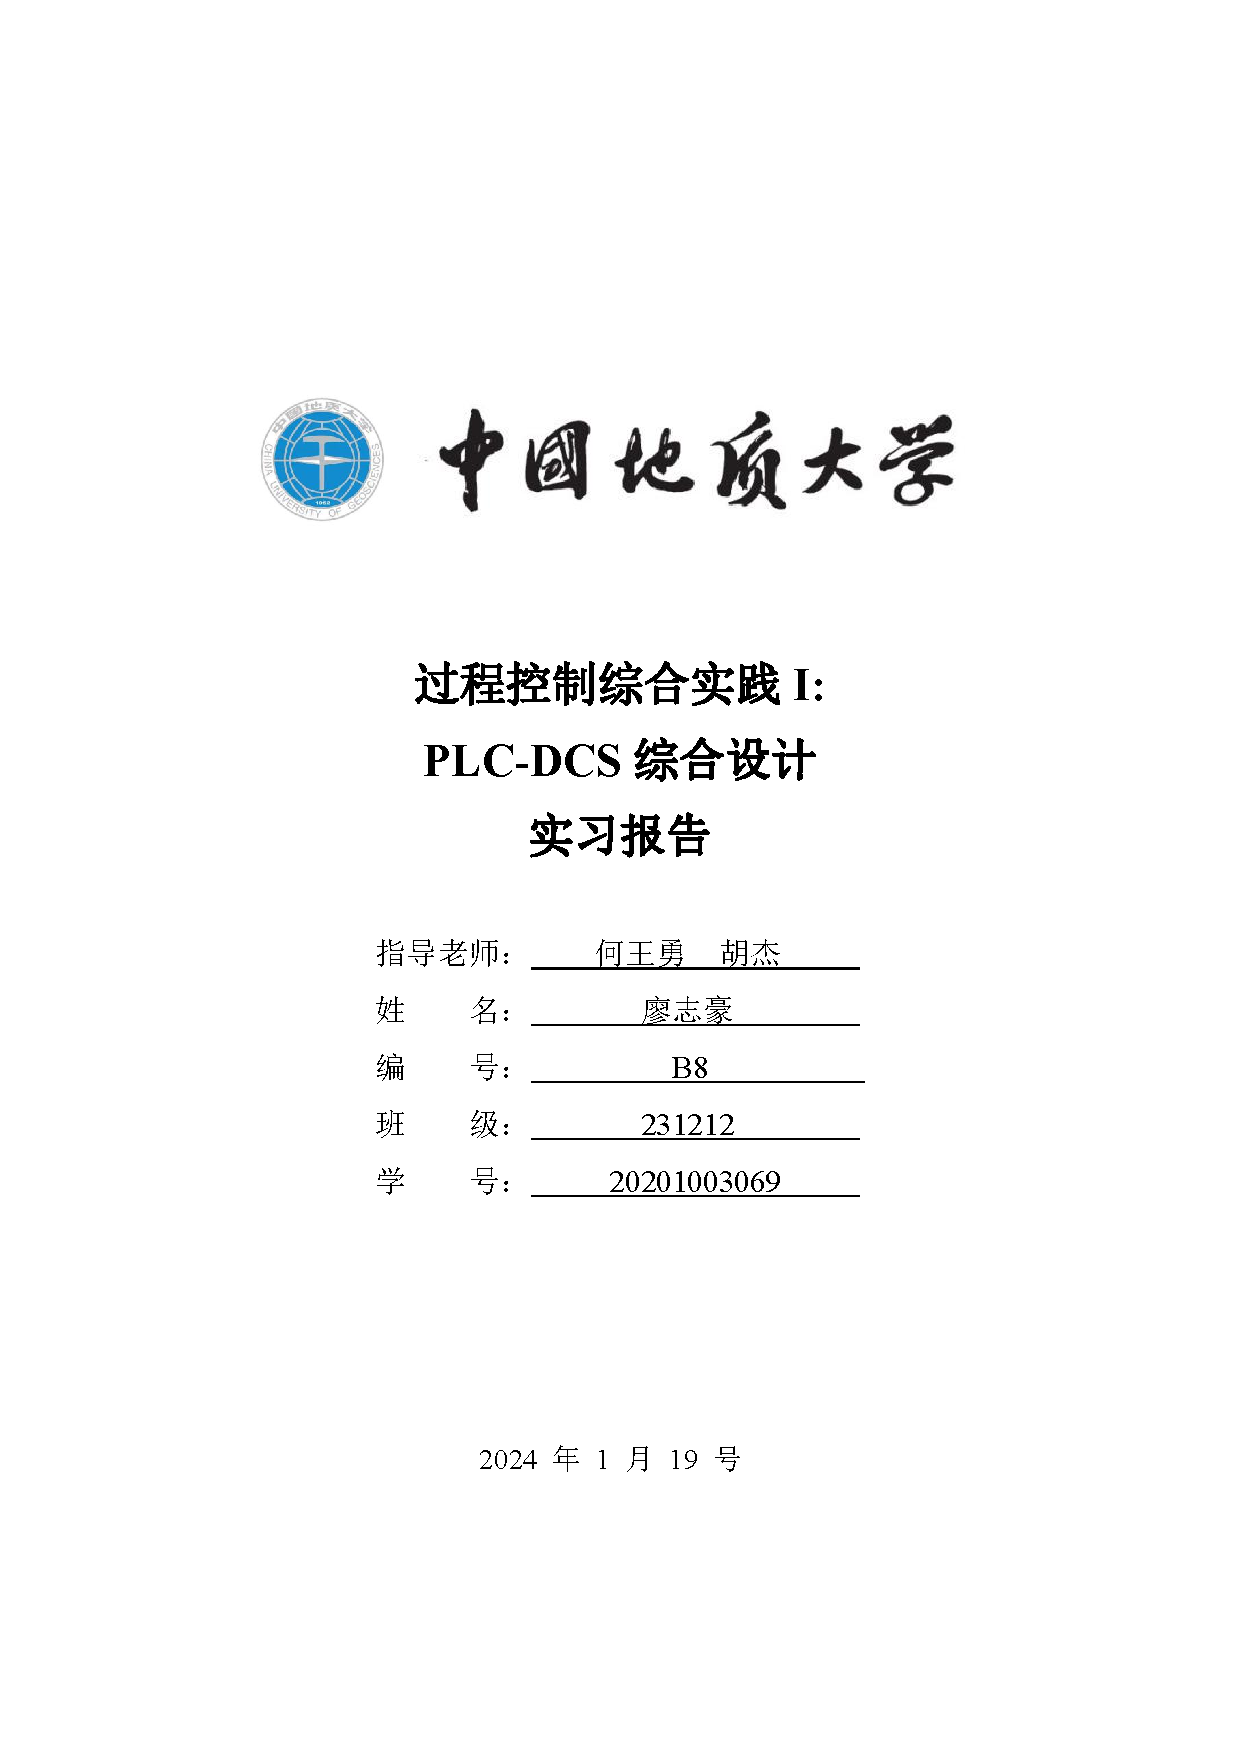
\includepdf[pages={1}]{cover.pdf}
% \end{titlepage}

% 生成目录
% \tableofcontents
% \cleardoublepage

% 导入图片
% \begin{figure}[H]
%     \centering % 居中 
%     % 图片文件的相对路径
%     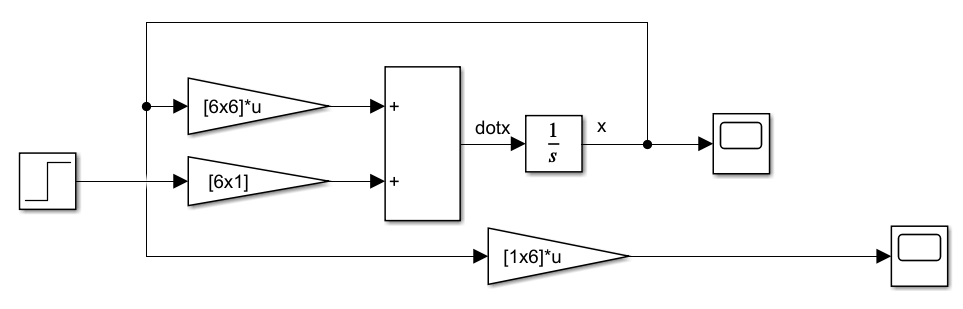
\includegraphics[width=.8\textwidth]{figure/exp1_1_model.png} 
%     \caption{Simulink模型} % caption是图片的标题
%     % \label{img} % 此处的label相当于一个图片的专属标志,目的是方便上下文的引用
% \end{figure}

% 导入代码
% \begin{lstlisting}
% a
% \end{lstlisting}

% 重置章节编号
% \setcounter{section}{0}

% \begin{table}[H] % 防止表格乱跑
% \centering % 居中
% \begin{tabular}{cccccc} % 指明列数
% 	\toprule % 顶部粗线
% 	序号 & 姓名 & 性别 & 年龄 & 身高/cm & 体重/kg \\
% 	\midrule % 中间细线
% 	1 & 张三 & M & 16 & 163 & 50 \\ % 每行末尾都要加换行符
% 	2 & 王红 & F & 15 & 159 & 47 \\
% 	3 & 李二 & M & 17 & 165 & 52 \\
% 	\bottomrule % 底部粗线
% \end{tabular}
% \caption{title} % 标题
% \end{table}

\begin{document}

\begin{titlepage}
% 封面信息
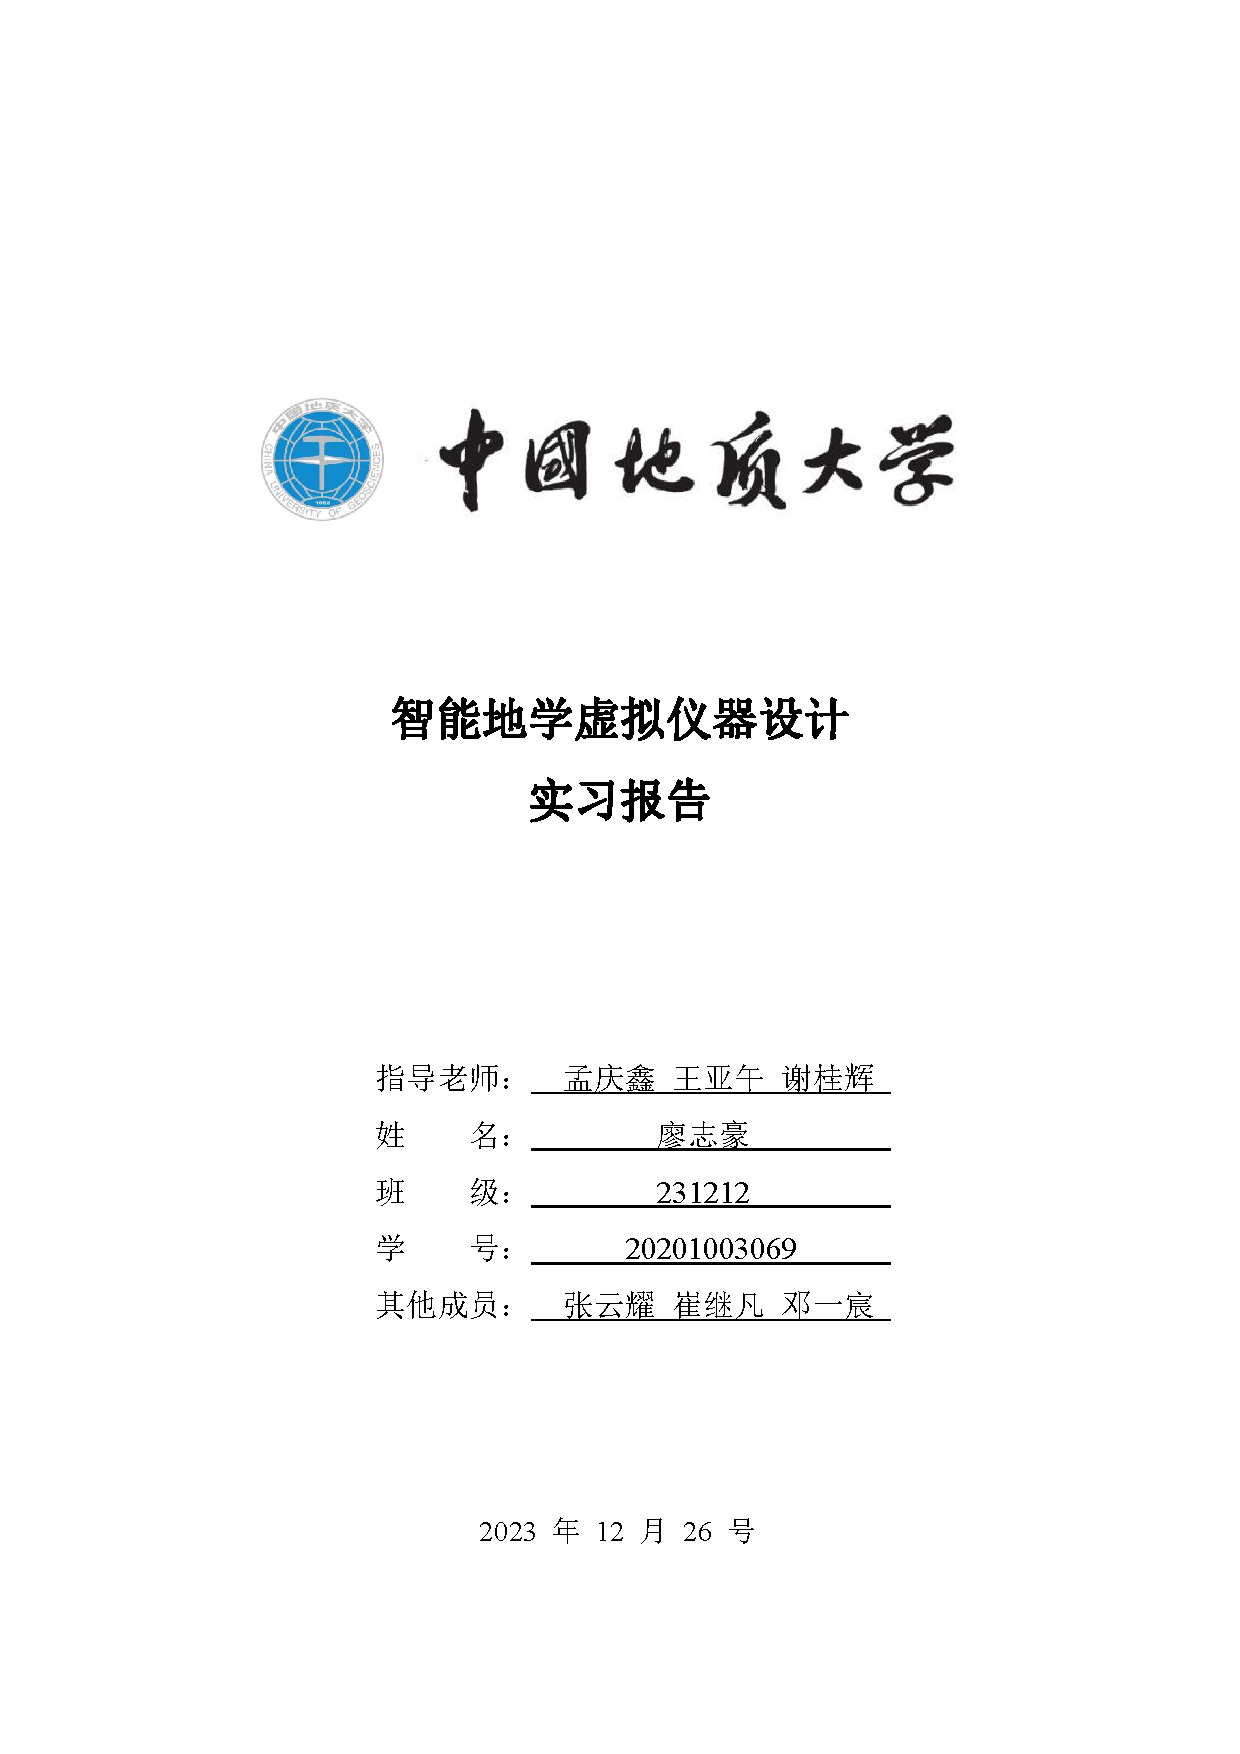
\includepdf[pages={1}]{./cover/cover.pdf}
\end{titlepage}

% 生成目录
\tableofcontents
\cleardoublepage

% 侧重点:labview部分

%
\section{实习目的与要求}
%%
\subsection{实习目的}
\begin{enumerate}
	\item 培养学生对嵌入式系统与地学虚拟仪器的分析和应用能力;
	\item 使用LabVIEW实验平台结合单片机等部件,构建嵌入式虚拟仪器的能力;
	\item 掌握配置LabVIEW实验平台和使用配套硬件开发装置的方法,熟悉嵌入式系统采样工作原理和工程开发流程。
\end{enumerate}



%%
\subsection{实习要求}
\begin{enumerate}
	\item 硬件功能模块设计:设计并制作一个功率驱动电路,用来放大来自单片机的信号。
	\item 软件功能模块设计:基于简单的通信协议,实现51单片机与LabVIEW上位机之间的串口通信。在此基础上,实现上位机指定频率和波形类型的方波信号输出(即主动源信号),以及ADC采集数据的上传。
	\item LabVIEW上位机系统:基于和51单片机的通信,提供两个功能模块:发射模块用于下发指令到单片机,实现对单片机发射信号的频率、波形类型的属性的设置;接收模块用于接收单片机回传的ADC数据并将信号以波形的形式显示在界面上。
	\item 地学虚拟仪器构建:整合上述各个功能模块,基于地学探测原理和相应的传感器,构建基于电法勘探的地学探测虚拟仪器。
\end{enumerate}

%%
\subsection{分工}
本次实习中,我和小组另一位同学主要负责单片机与LabVIEW上位机的相关工作,包括程序调试、通信测试等。此外,我们还负责综合实践部分地学虚拟仪器的构建和调试。

%
\section{系统介绍}
%%
\subsection{系统结构}
本次实习主要完成基于电法测量的地学虚拟仪器系统,整个系统大致由三
个部分组成,即LabVIEW上位机、51单片机系统以及其他外围电路。其中LabVIEW上位机用于下发指令到单片机系统,同时接收来自单片机的数据用于显示采集信号的波形;51单片机系统用于根据上位机的指令,发射指定频率和波形类型的方波信号,以及将ADC采集到的信号数据上传至上位机;外围电路则负责一些特定任务,包括模数转换电路和功率放大电路等。系统的大致结构如下图所示:
\begin{figure}[H]
    \centering % 居中 
    % 图片文件的相对路径
    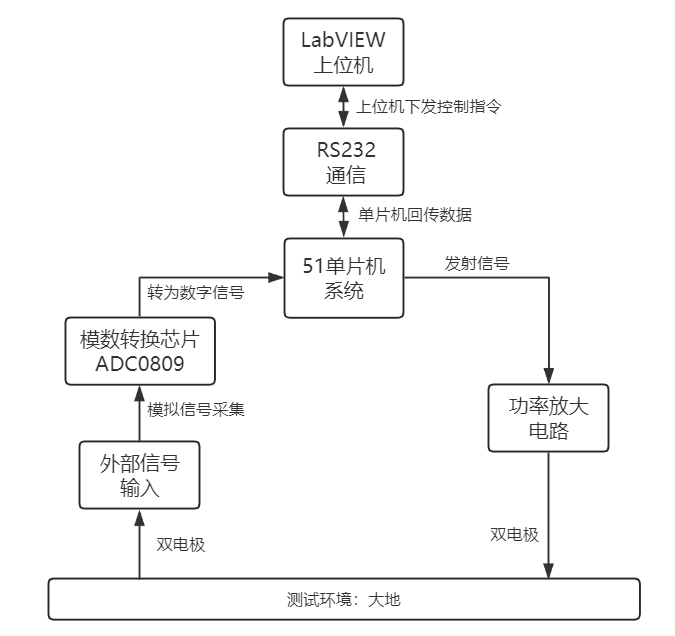
\includegraphics[width=.6\textwidth]{figure/系统结构.png} 
    \caption{系统结构示意图} % caption是图片的标题
    % \label{img} % 此处的label相当于一个图片的专属标志,目的是方便上下文的引用
\end{figure}

%%
\subsection{地学虚拟仪器:电法测量基本原理}
如下图所示,向AB两点施加激励信号,则AB之间会产生相应的电场,该电场进一步产生磁场。其中的地下介质在磁场作用下会发生极化现象。对于高电阻率的介质,其极化现象不明显,AB两点间的电场基本呈半圆形,磁场垂直于电场且均匀分布;对于低电阻率的介质,其在磁场作用下会发生极化产生涡流,涡流反过来会影响磁场的分布。从而可以知道,两电极MN之间的电压会随着MN两点之间介质电阻率的不同而发生变化,且容易得出两者之间的变化趋势是相同的。这也就意味着,当在MN两电极之间放入一个电阻率很低的介质,比如金属块时,两电极之间的电压信号将会出现明显下降。这就是电法测量的基本原理。
\begin{figure}[H]
    \centering % 居中 
    % 图片文件的相对路径
    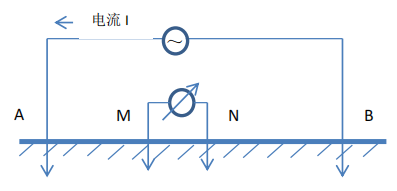
\includegraphics[width=.5\textwidth]{figure/电法测量原理图.png} 
    \caption{电法测量原理图} % caption是图片的标题
    % \label{img} % 此处的label相当于一个图片的专属标志,目的是方便上下文的引用
\end{figure}

%
\section{硬件功能模块设计}
由于单片机IO口输出的方波信号没有足够的驱动能力,因此本次实习中需要设计并制作一个功率驱动电路以实现对单片机信号的功率放大。放大后的信号将施加在发射电极上,以实现主动源信号发射和探测。

本次设计和制作的功率驱动电路主要包含四个部分,分别是:隔离电路、MOSFET驱动电路、全桥驱动电路和供电电路。下面是我们小组制作的功率驱动电路板:
\begin{figure}[H]
    \centering % 居中 
    % 图片文件的相对路径
    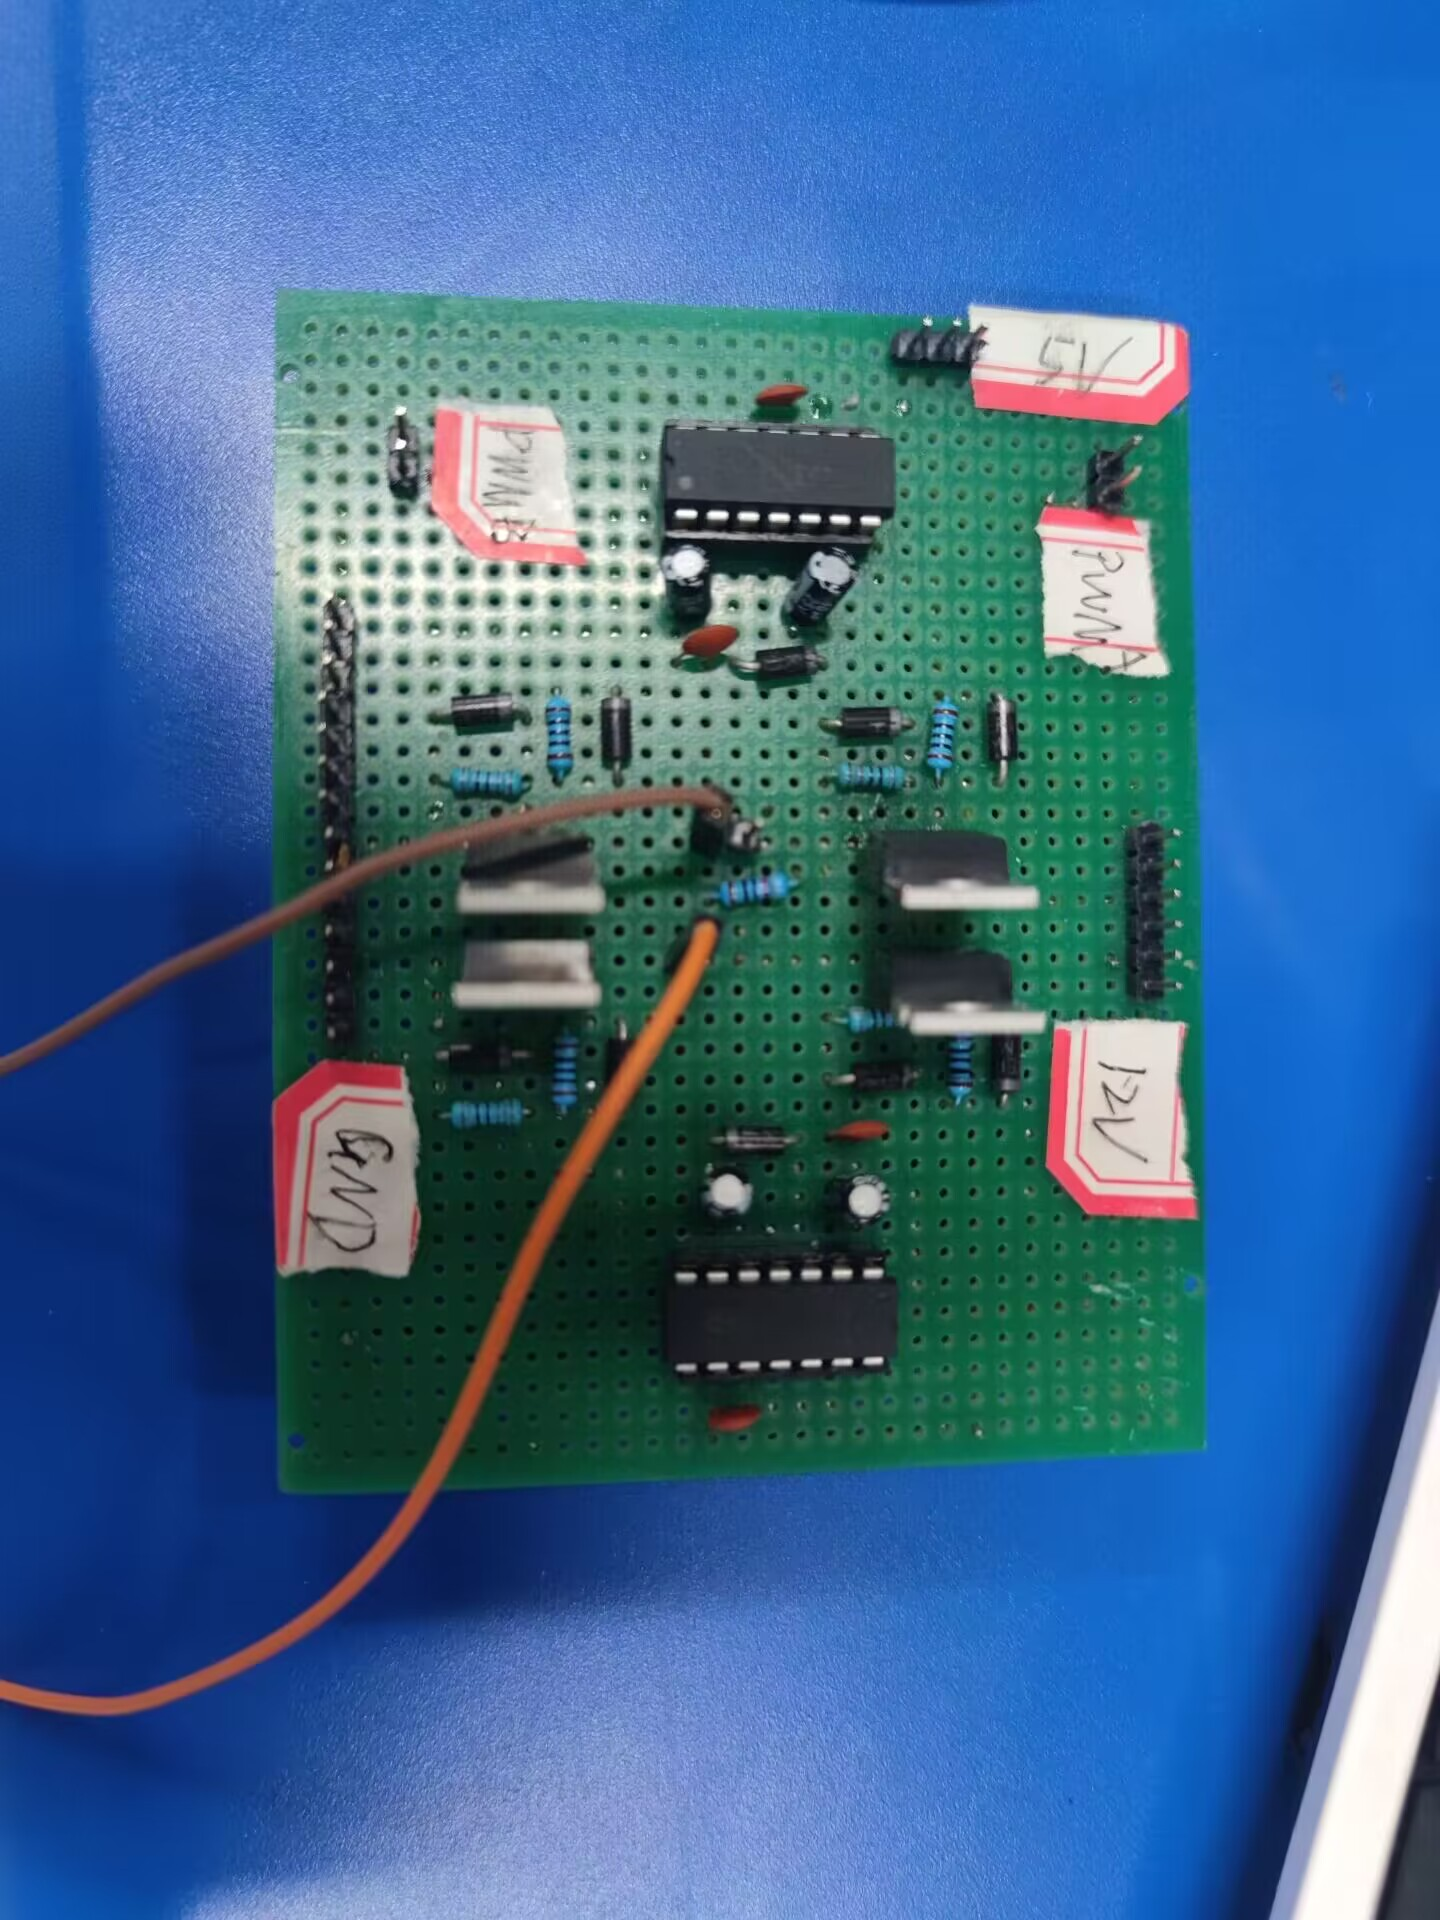
\includegraphics[width=.5\textwidth]{figure/功率驱动板.jpg} 
    \caption{功率驱动电路板} % caption是图片的标题
    % \label{img} % 此处的label相当于一个图片的专属标志,目的是方便上下文的引用
\end{figure}

%%
\subsection{隔离电路}
隔离电路的主要作用是将控制电路与后续电路进行隔离。本次实习使用单片机作为控制电路,电压较低;而一般来说驱动电路的电压较高,为防止控制电路被意外烧毁,需要在控制电路和驱动电路之间加入一个隔离电路。这里我们采用隔离电路的通常实现方式,使用光电隔离芯片6N137构成隔离电路,其电路原理图如下:
\begin{figure}[H]
    \centering % 居中 
    % 图片文件的相对路径
    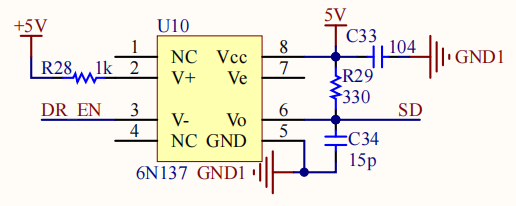
\includegraphics[width=.8\textwidth]{figure/隔离电路.png} 
    \caption{6N137隔离电路原理图} % caption是图片的标题
    % \label{img} % 此处的label相当于一个图片的专属标志,目的是方便上下文的引用
\end{figure}

%%
\subsection{MOSFET驱动电路}
功率驱动电路的主体是一个典型的全桥驱动电路,通过MOSFET器件构成,这就涉及到MOSFET的驱动问题。一般情况下,单片机输出的电压信号较弱,不能直接用于驱动大功率的MOSFET。因此我们需要设计针对MOSFET的驱动电路,将来自单片机的控制信号进行放大后再用于驱动MOSFET。MOSFET的驱动电路实现可以采用IR2110S芯片,以下是MOSFET驱动电路的原理图:
\begin{figure}[H]
    \centering % 居中 
    % 图片文件的相对路径
    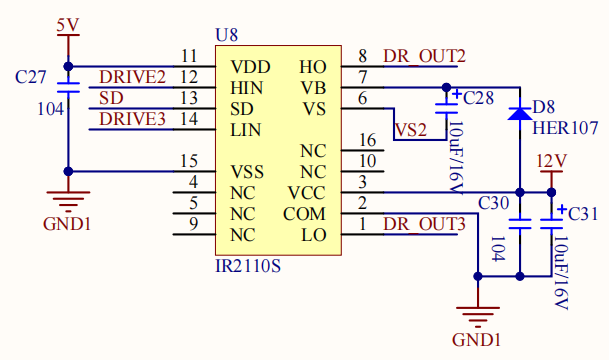
\includegraphics[width=.8\textwidth]{figure/MOSFET驱动.png} 
    \caption{MOSFET驱动电路原理图} % caption是图片的标题
    % \label{img} % 此处的label相当于一个图片的专属标志,目的是方便上下文的引用
\end{figure}

%%
\subsection{全桥驱动电路}
如下图所示为全桥驱动电路的原理图。该驱动电路由4个N沟道MOSFET构成,通过输入PWM信号以控制桥臂的通断情况。经测试验证,通过输入特定的PWM信号,该电路可以连续输出双极性的方波交流电。
\begin{figure}[H]
    \centering % 居中 
    % 图片文件的相对路径
    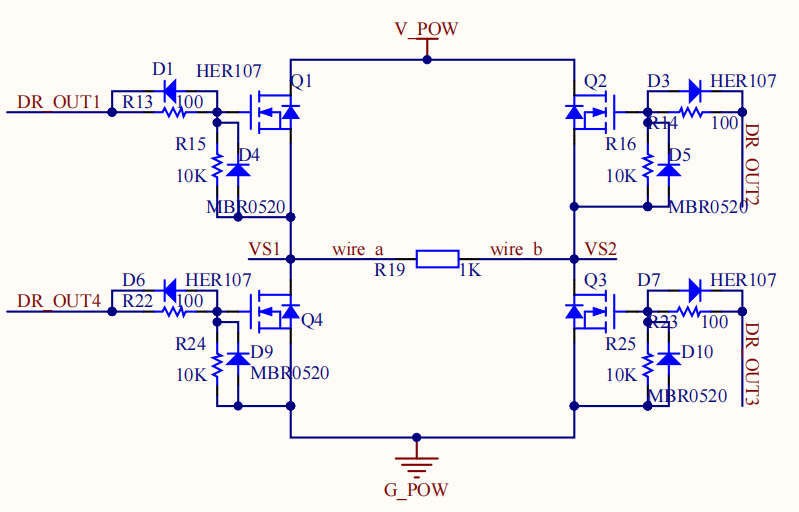
\includegraphics[width=.8\textwidth]{figure/全桥驱动电路.png} 
    \caption{全桥驱动电路原理图} % caption是图片的标题
    % \label{img} % 此处的label相当于一个图片的专属标志,目的是方便上下文的引用
\end{figure}
\begin{figure}[H]
    \centering % 居中 
    % 图片文件的相对路径
    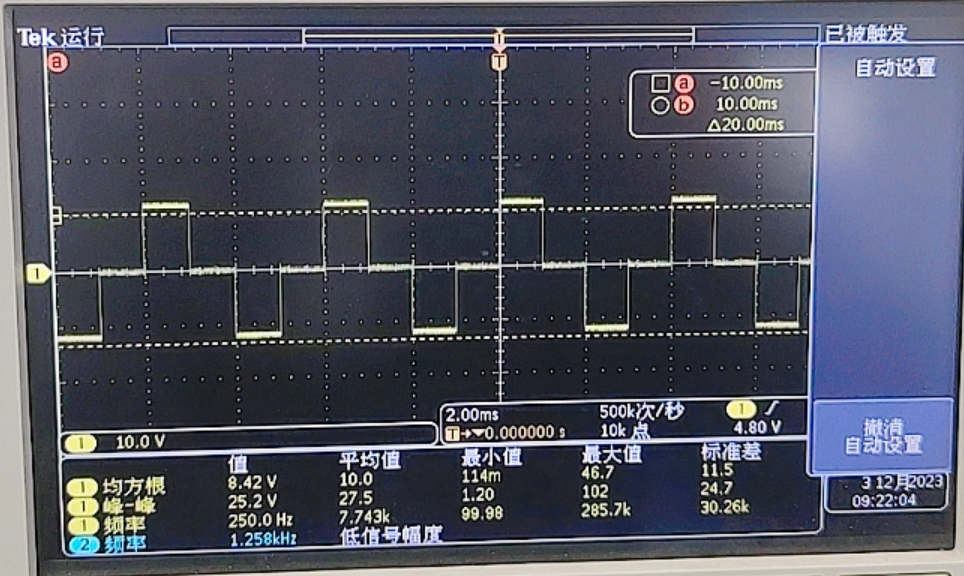
\includegraphics[width=.6\textwidth]{figure/双极性方波.png} 
    \caption{双极性方波效果图} % caption是图片的标题
    % \label{img} % 此处的label相当于一个图片的专属标志,目的是方便上下文的引用
\end{figure}

%%
\subsection{供电电路}
供电电路用于提供其他电路所需的5V和12V电源,其电路原理图如下图所示。端口VIN输入电压范围为12V~18V,经过WRB1212稳压后得到12V电压,在经过WRB1205后得到5V电压。
\begin{figure}[H]
    \centering % 居中 
    % 图片文件的相对路径
    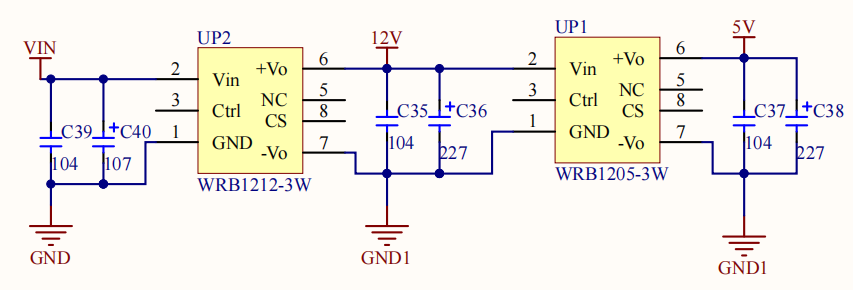
\includegraphics[width=.8\textwidth]{figure/电源电路.png} 
    \caption{供电电路原理图} % caption是图片的标题
    % \label{img} % 此处的label相当于一个图片的专属标志,目的是方便上下文的引用
\end{figure}

%
\section{软件功能模块设计}
%%
\subsection{单片机实验平台介绍}
本次实习使用的单片机为基于伟福LAB9000实验箱的51单片机仿真系统,可以直接作为51单片机使用,并且支持使用Keil软件进行程序开发。
\begin{figure}[H]
    \centering % 居中 
    % 图片文件的相对路径
    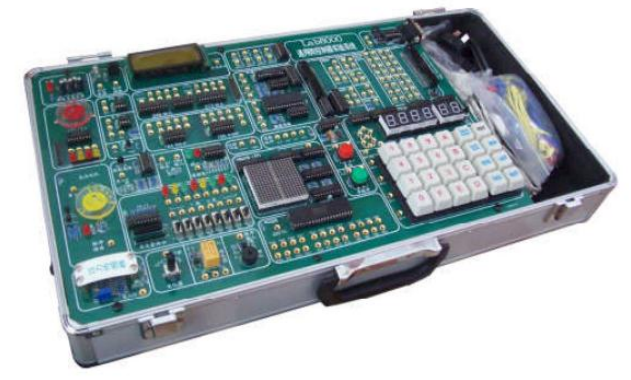
\includegraphics[width=.6\textwidth]{figure/实验箱.png} 
    \caption{伟福LAB9000实验箱} % caption是图片的标题
    % \label{img} % 此处的label相当于一个图片的专属标志,目的是方便上下文的引用
\end{figure}

此外,在本次实习所要求构建的地学虚拟仪器系统中,单片机处理的工作包括信号的发生以及信号采集和上传。为便于调试,我们在实习过程中分别使用两套单片机系统以分别实现上述两种功能。

%%
\subsection{信号波形发生}
%%% 
\subsubsection{原理介绍}
对于波形信号的发生,我们主要利用51单片机产生频率可调的PWM波。具体来说,我们使用LabVIEW上位机系统,通过RS232通讯给单片机下发指令,单片机在接收到指令后进行数据解析,解析完成后得到波形产生的启停、波形频率和波形类型等信息。然后,单片机将根据指令要求从特定的IO口输出指定电平信号到放大电路,同时控制高低电平时间以达到调频效果。这样就能使单片机输出我们想要的特定频率和类型的方波信号。在这个过程中,信号的传递方向可以参考下图:
\begin{figure}[H]
    \centering % 居中 
    % 图片文件的相对路径
    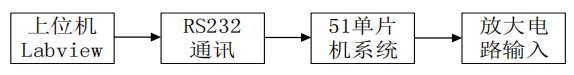
\includegraphics[width=.8\textwidth]{figure/信号波形产生-信号方向示意.png} 
    \caption{信号波形发生过程的信号传递方向} % caption是图片的标题
    % \label{img} % 此处的label相当于一个图片的专属标志,目的是方便上下文的引用
\end{figure}

%%% 
\subsubsection{实验平台搭建}
信号波形产生的实验平台搭建主要涉及到一些接线工作:将电脑通过RS232串口线连接到实验箱的232接口,实验箱232接口的TXD和RXD端口分别与IO口P3.1和P3.0相连,信号输出端口P1.0和P1.1连接到放大电路对应的输入端。具体的接线方式见下表:
\begin{table}[H] % 防止表格乱跑
\centering % 居中
\begin{tabular}{ccc} % 指明列数
	\toprule % 顶部粗线
	接线序号 & 接线端1 & 接线端2 \\
	\midrule % 中间细线
	1 & P1.0 & 输出口1 \\
	2 & P1.1 & 输出口2 \\
	3 & 电脑 & 232 \\
	4 & P3.0 & 232 RXD \\
	5 & P3.1 & 232 TXD \\
	\bottomrule % 底部粗线
\end{tabular}
\caption{信号波形产生实验-接线方式} % 标题
\end{table}

%%% 
\subsubsection{实验程序框图}
信号波形产生的程序框图如下图所示。首先对串口、定时器T0进行初始化和设定初值,在循环中对数据进行修改。当上位机下发指令时,串口接收数据产生中断,将数据存储并将接收数据完成标志位置1,然后返回主函数。接着对指令进行解析,得到波形输出启停、波形类型、方波频率等信息,并对定时器进行相应设置。打开定时器T0后,定时器T0会每隔1000us进入一次中断,并在中断里完成一次计数,当计数值等于某个指定的数值时就让输出的电平翻转一次,这样就实现了特定频率信号波形的输出。
\begin{figure}[H]
    \centering % 居中 
    % 图片文件的相对路径
    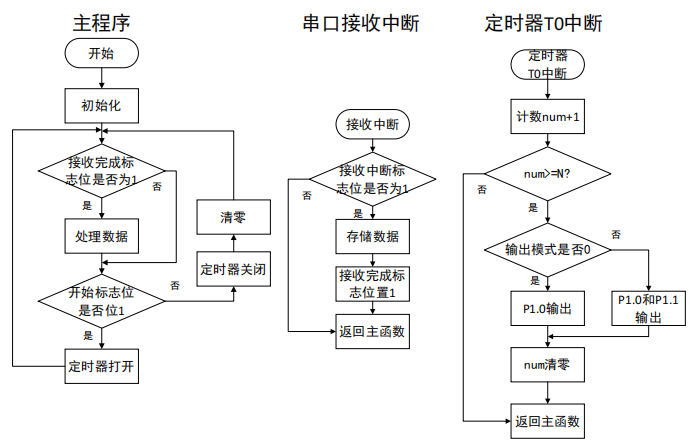
\includegraphics[width=.8\textwidth]{figure/信号波形产生-程序框图.png} 
    \caption{信号波形产生程序框图} % caption是图片的标题
    % \label{img} % 此处的label相当于一个图片的专属标志,目的是方便上下文的引用
\end{figure}

%%
\subsection{ADC数据上传}
%%% 
\subsubsection{原理介绍}
ADC数据上传过程如下图所示。51单片机系统在采集到外部模拟电信号后,会将信号输入到模数转换芯片ADC0809中进行处理,通过逐次逼近的方式将模拟电信号转换为数字信号,并传送给51单片机;单片机系统进而通过RS232通信将数据实时发送到LabVIEW上位机中,并在上位机界面上显示出对应的波形信号图。
\begin{figure}[H]
    \centering % 居中 
    % 图片文件的相对路径
    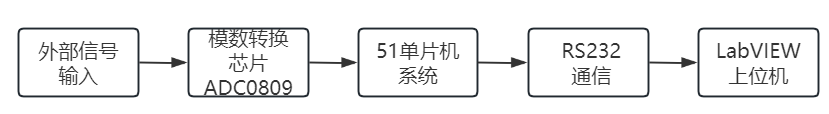
\includegraphics[width=.8\textwidth]{figure/ADC数据上传.png} 
    \caption{ADC数据上传过程} % caption是图片的标题
    % \label{img} % 此处的label相当于一个图片的专属标志,目的是方便上下文的引用
\end{figure}

%%% 
\subsubsection{实验平台搭建}
电脑通过RS232串口线连接到实验箱的232接口,232处的TXD和RXD分别与IO口P3.1和P3.0相连;在模数转换部分将外部信号输入连接到IN0,将AD\_CS 连接到片选地址CS0;在扩展引脚部分,将8255\_CS连接到片选地址CS1,最后将PA依此连接到LED灯。具体的接线方式见下表:
\begin{table}[H] % 防止表格乱跑
\centering % 居中
\begin{tabular}{cccccc} % 指明列数
	\toprule % 顶部粗线
	接线序号 & 接线端1 & 接线端2 & 接线序号 & 接线端1 & 接线端2 \\
	\midrule % 中间细线
	1 & P3.0 & 232RXD & 8 & PA1 & L1 \\
	2 & P3.1 & 232TXD & 9 & PA2 & L2 \\
	3 & 电脑 & 232 & 10 & PA3 & L3 \\
	4 & IN0 & 输入口 & 11 & PA4 & L4 \\
	5 & CS0 & AD\_CS & 12 & PA5 & L5 \\
	6 & CS1 & 8255\_CS & 13 & PA6 & L6 \\
	7 & PA0 & L0 & 14 & PA7 & L7 \\
	\bottomrule % 底部粗线
\end{tabular}
\caption{ADC数据上传实验-接线方式} % 标题
\end{table}

%%% 
\subsubsection{实验程序框图}
ADC数据上传的程序框图如下图所示。首先对串口和定时器T0进行初始化和设定初值,在循环中等待定时器T0产生中断并将标志位置1,当标志位置1时就将ADC采集到的数据上传至上位机。
\begin{figure}[H]
    \centering % 居中 
    % 图片文件的相对路径
    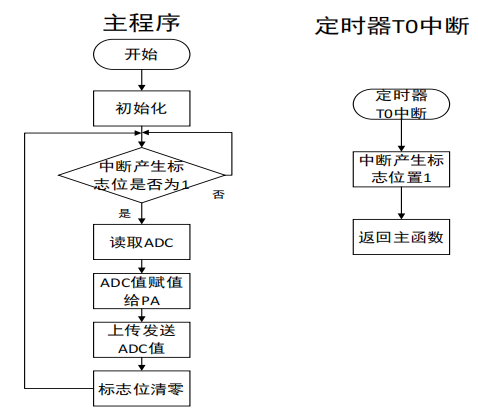
\includegraphics[width=.6\textwidth]{figure/ADC数据上传-程序框图.png} 
    \caption{ADC数据上传程序框图} % caption是图片的标题
    % \label{img} % 此处的label相当于一个图片的专属标志,目的是方便上下文的引用
\end{figure}

%
\section{基于LabVIEW的上位机系统}
在本次实习中,我们使用基于LabVIEW开发的地学虚拟仪器电法勘测发射采集一体化系统作为51单片机的上位机系统。该系统主要包含两大功能模块,分别是地学虚拟仪器发射模块和地学虚拟仪器采集模块。这两大功能模块分别实现了对单片机发射信号的频率、波形类型等属性的设置,和读取单片机采集到的ADC电压数据并以波形的形式显示在上位机界面中。

%%
\subsection{界面设计及功能介绍}
%%%
\subsubsection{地学虚拟仪器发射模块}
%%%%
\paragraph{界面设计}~{}

地学虚拟仪器发射模块的界面设计如下图所示:
\begin{figure}[H]
    \centering % 居中 
    % 图片文件的相对路径
    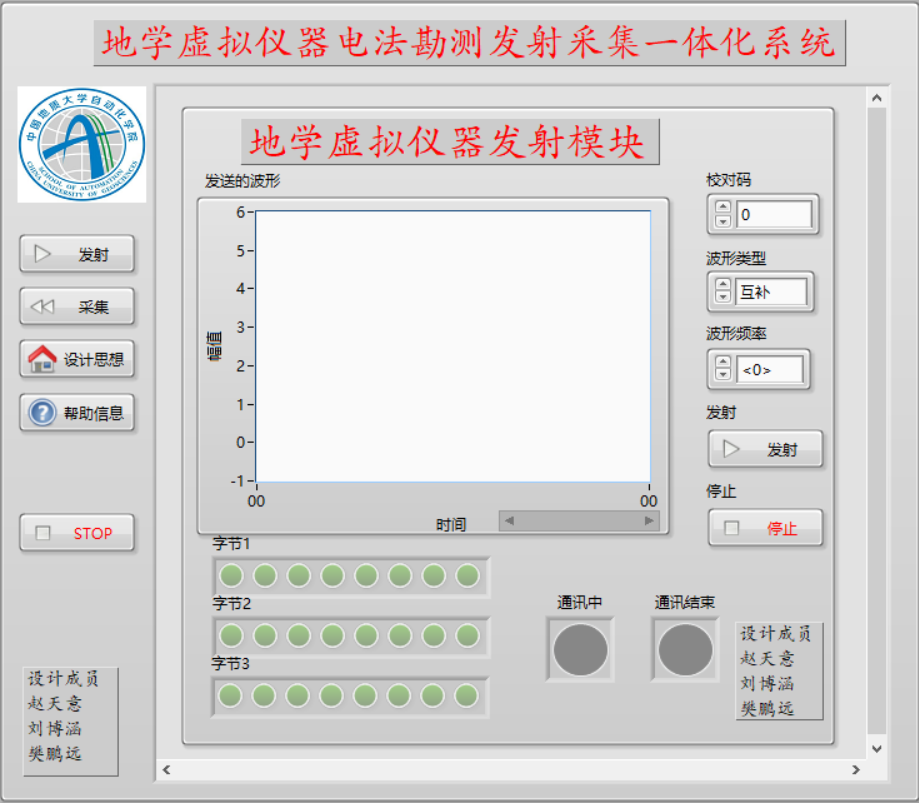
\includegraphics[width=.6\textwidth]{figure/发射界面.png} 
    \caption{发射模块的界面设计} % caption是图片的标题
    % \label{img} % 此处的label相当于一个图片的专属标志,目的是方便上下文的引用
\end{figure}

%%%%
\paragraph{功能介绍}~{}

发射模块可以实现10Hz~1kHz频域内方波信号的产生,调频范围广,且精度较高,总体偏差在3\%以内;支持输出互补和非互补两种波形信号;使用8位二进制校验码,用于上位机与下位机的数据校对,避免在野外测试场景下因传输距离过长而导致的数据出错问题;此外在发射模块界面中还添加了指示灯用于指示上位机与下位机通信的正常进行和停止,当发送成功后,“通讯中”指示灯将会闪烁一次,当结束通信以后,“通讯结束指示灯”将会闪烁两次。

另外,该上位机系统采用了较为简单的传输协议。采用3个字节作为一个数据帧进行传输,前两个字节包含有运行状态、波形类型和信号频率等信息,最后一个字节作为校验码。在发射模块的前面板上放置有3个8位指示灯,可以非常直观地查看上位机发送的数据包。

%%%%
\paragraph{测试}~{}

使用LabVIEW上位机控制51单片机输出指定频率的互补波形,效果如下:
\begin{figure}[htbp]
	\centering
	\begin{minipage}{0.49\linewidth}
		\centering
		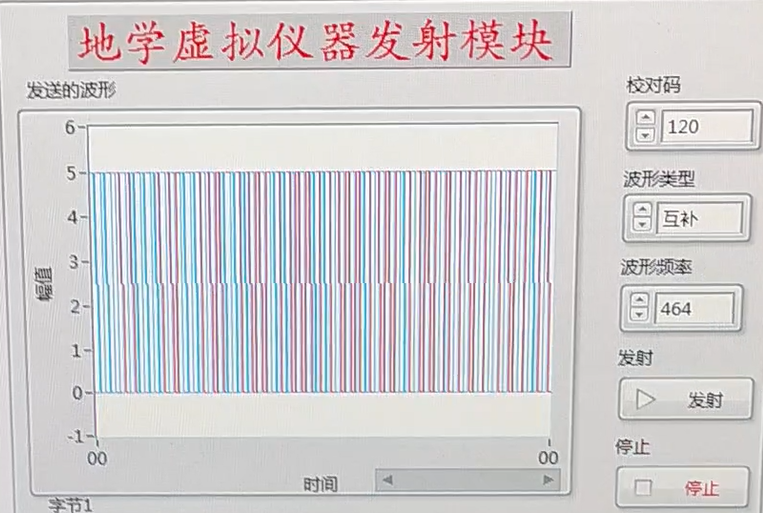
\includegraphics[width=0.9\linewidth]{figure/发射模块测试.png}
		\caption{发射模块测试}
		\label{label1} %文中引用该图片代号
	\end{minipage}
	%\qquad
	\begin{minipage}{0.49\linewidth}
		\centering
		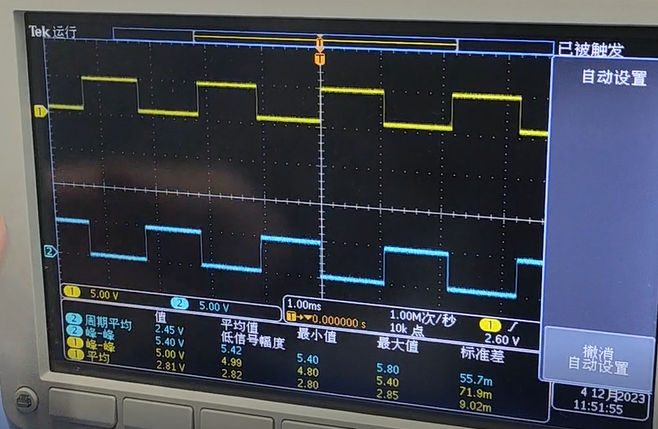
\includegraphics[width=0.9\linewidth]{figure/互补波形.png}
		\caption{单片机输出的互补波形}
		\label{label2} %文中引用该图片代号
	\end{minipage}
\end{figure}


%%%
\subsubsection{地学虚拟仪器采集模块}
%%%%
\paragraph{界面设计}~{}

地学虚拟仪器采集模块的界面设计如下图所示:
\begin{figure}[H]
    \centering % 居中 
    % 图片文件的相对路径
    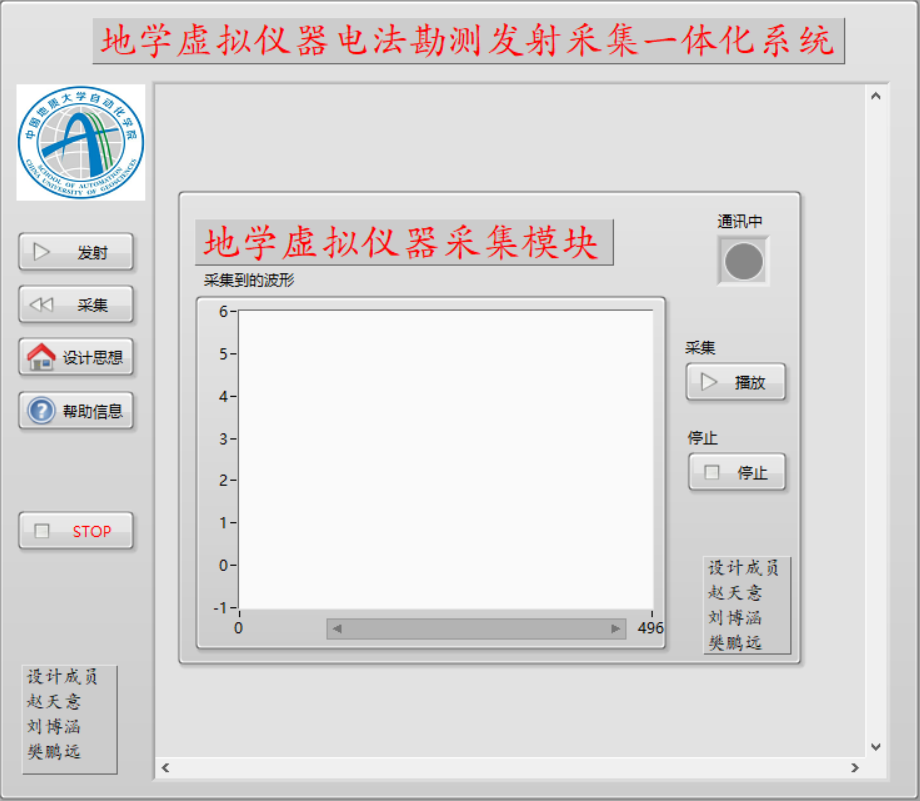
\includegraphics[width=.6\textwidth]{figure/采集界面.png} 
    \caption{采集模块的界面设计} % caption是图片的标题
    % \label{img} % 此处的label相当于一个图片的专属标志,目的是方便上下文的引用
\end{figure}

%%%%
\paragraph{功能介绍}~{}

通过采集模块,上位机可以接收下位机(即51单片机)传来的波形信号,并将波形显示在界面上。在上位机与下位机连接成功,通信正常的情况下,点击界面的“播放”按键即可观察到波形;点击界面的“停止”按键可以停止波形显示,方便对波形进行查看。此外,界面上还设置了一个指示灯用于提示通讯是否正常。

%%%%
\paragraph{测试}~{}

将实验箱的ADC采集端口连接至一个电位器上,通过连续调节电位器,可以在LabVIEW上位机上观测到相应的电信号波形变化情况:
\begin{figure}[H]
    \centering % 居中 
    % 图片文件的相对路径
    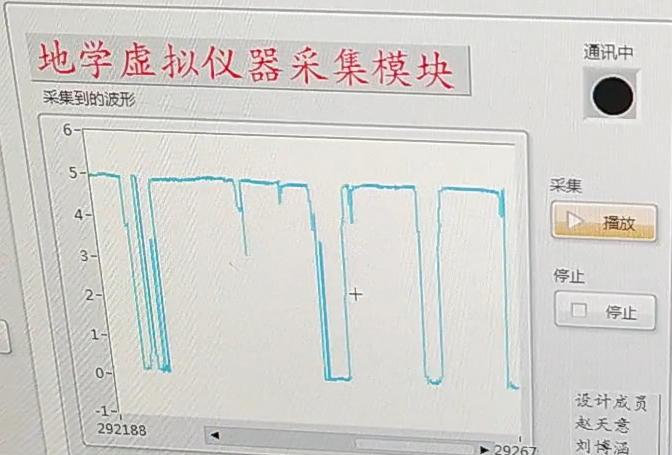
\includegraphics[width=.6\textwidth]{figure/采集模块测试.png} 
    \caption{采集模块测试} % caption是图片的标题
    % \label{img} % 此处的label相当于一个图片的专属标志,目的是方便上下文的引用
\end{figure}

%%
\subsection{LabVIEW程序设计}
本次实习使用基于LabVIEW开发的上位机系统,其实现的功能包括上位机与单片机通过串口进行数据交互、上位机发送激励信号指令到单片机,以及显示来自单片机的回传数据等。
%%%
\subsubsection{采集模块的实现}
上位机系统中采集功能模块的LabVIEW程序如下:
\begin{figure}[H]
    \centering % 居中 
    % 图片文件的相对路径
    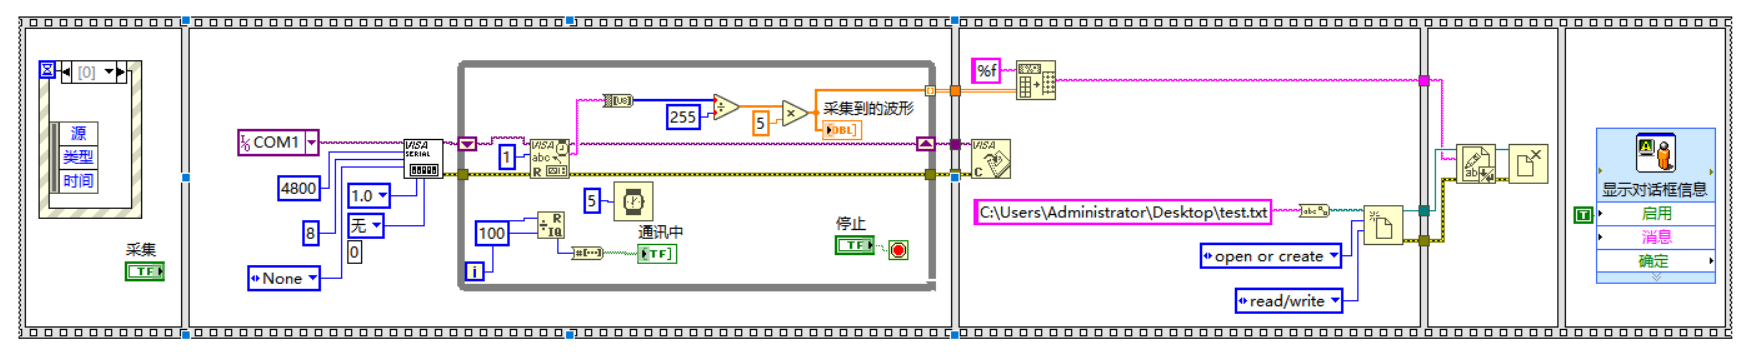
\includegraphics[width=1\textwidth]{figure/采集模块-程序.png} 
    \caption{采集模块程序图} % caption是图片的标题
    % \label{img} % 此处的label相当于一个图片的专属标志,目的是方便上下文的引用
\end{figure}
该程序主要由顺序程序结构和事件结构组成。在事件结构中,可以通过改变采集按键的值来改变事件。基于接口软件VISA实现串口的配置、数据流的读取和关闭等功能;通过波形图表控件完成信号的转换和显示。此外,该程序还使用了LabVIEW的文件处理功能,以方便数据处理。

%%%
\subsubsection{发射模块的实现}
发射功能模块的LabVIEW程序如下:
\begin{figure}[H]
    \centering % 居中 
    % 图片文件的相对路径
    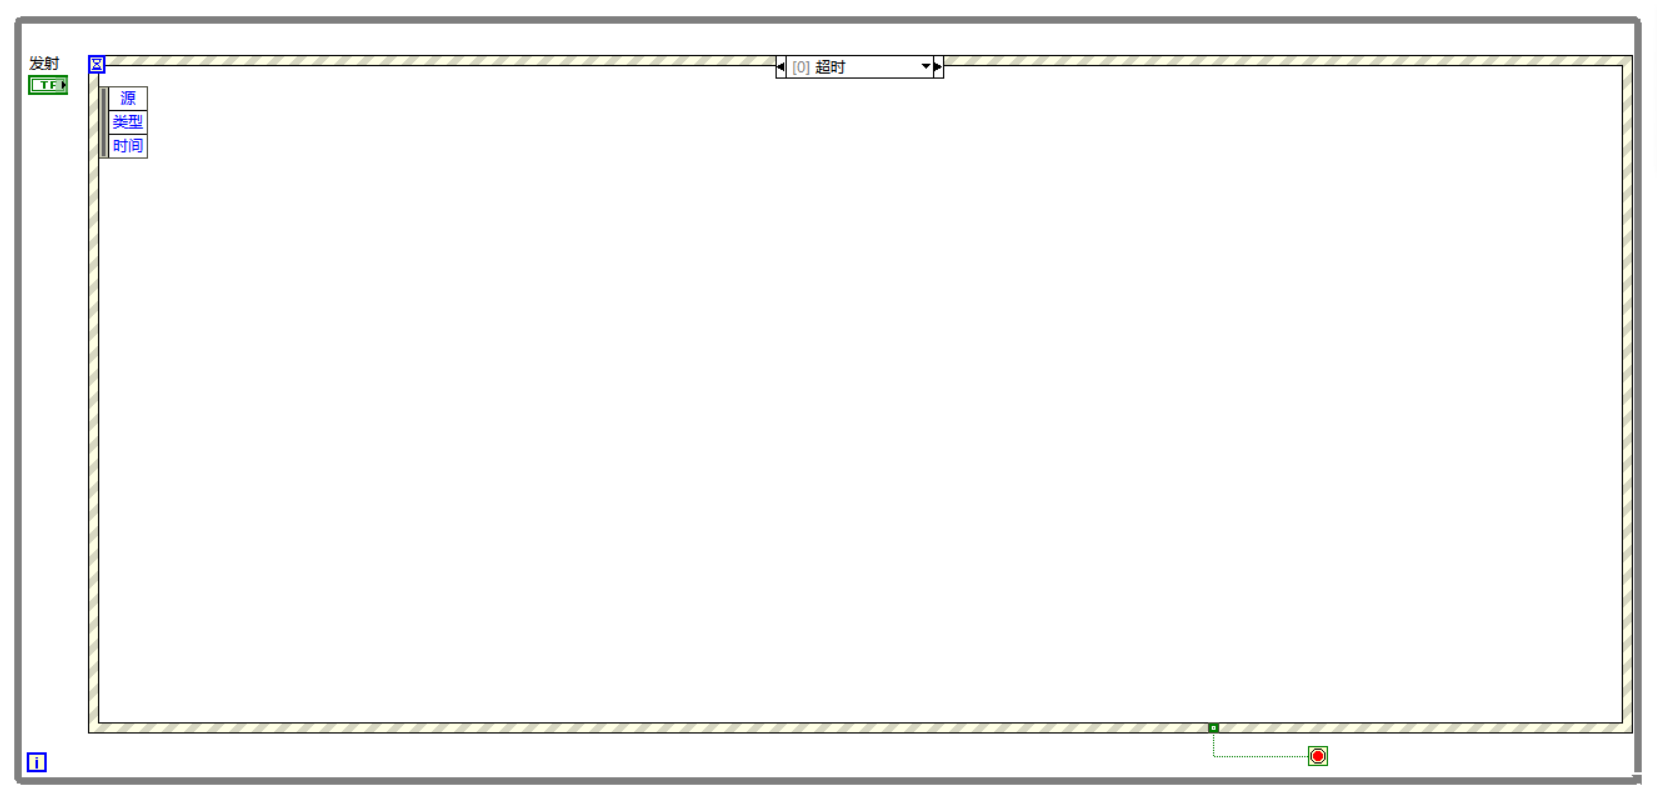
\includegraphics[width=1\textwidth]{figure/发射模块-程序0.png} 
    \caption{发射模块程序图[0]} % caption是图片的标题
    % \label{img} % 此处的label相当于一个图片的专属标志,目的是方便上下文的引用
\end{figure}
\begin{figure}[H]
    \centering % 居中 
    % 图片文件的相对路径
    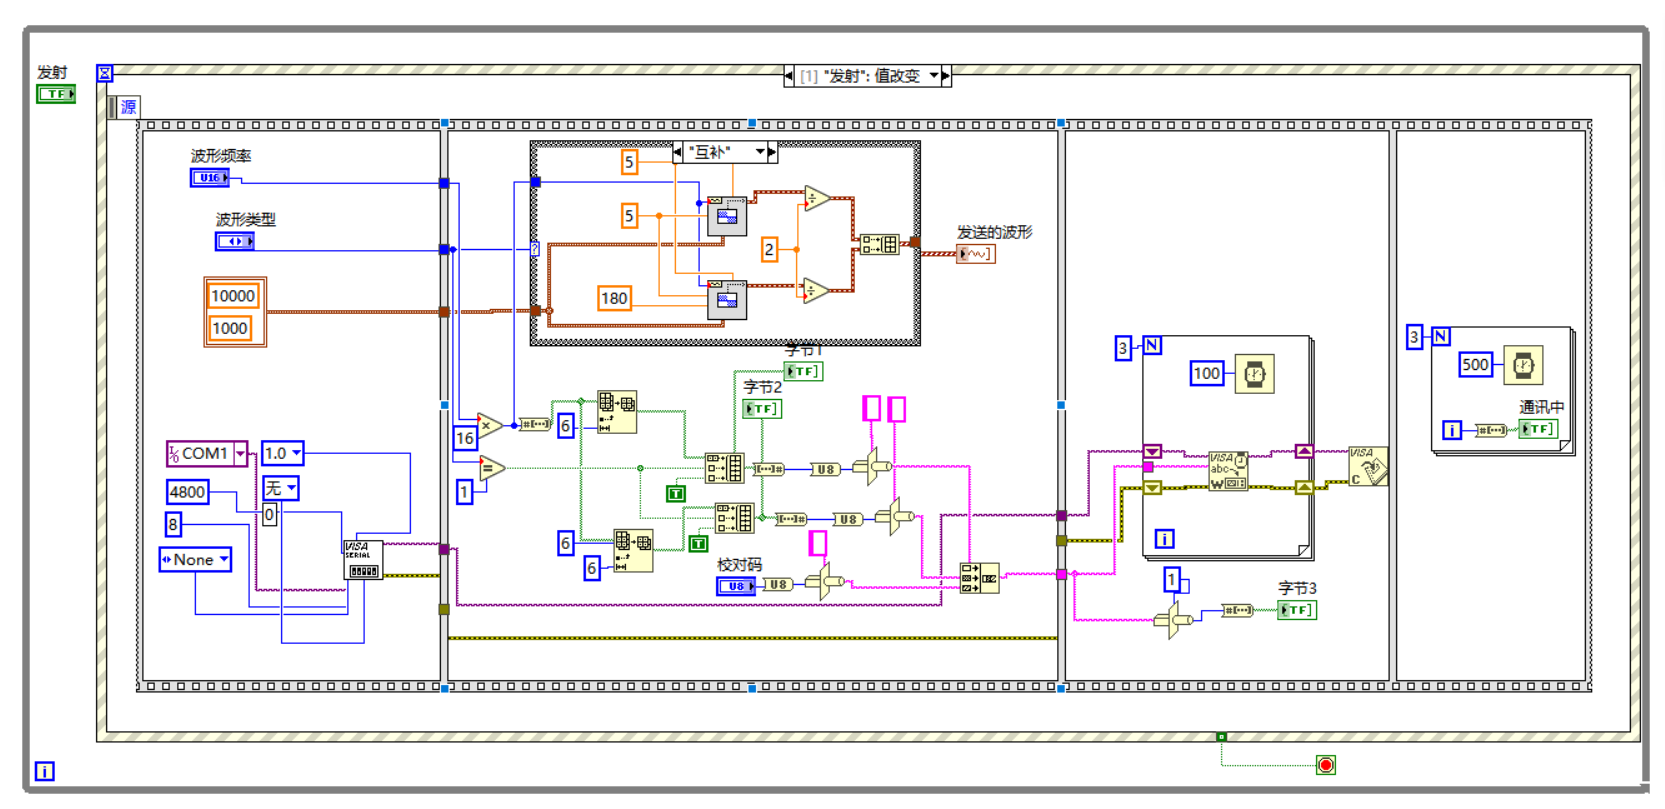
\includegraphics[width=1\textwidth]{figure/发射模块-程序1.png} 
    \caption{发射模块程序图[1]} % caption是图片的标题
    % \label{img} % 此处的label相当于一个图片的专属标志,目的是方便上下文的引用
\end{figure}
\begin{figure}[H]
    \centering % 居中 
    % 图片文件的相对路径
    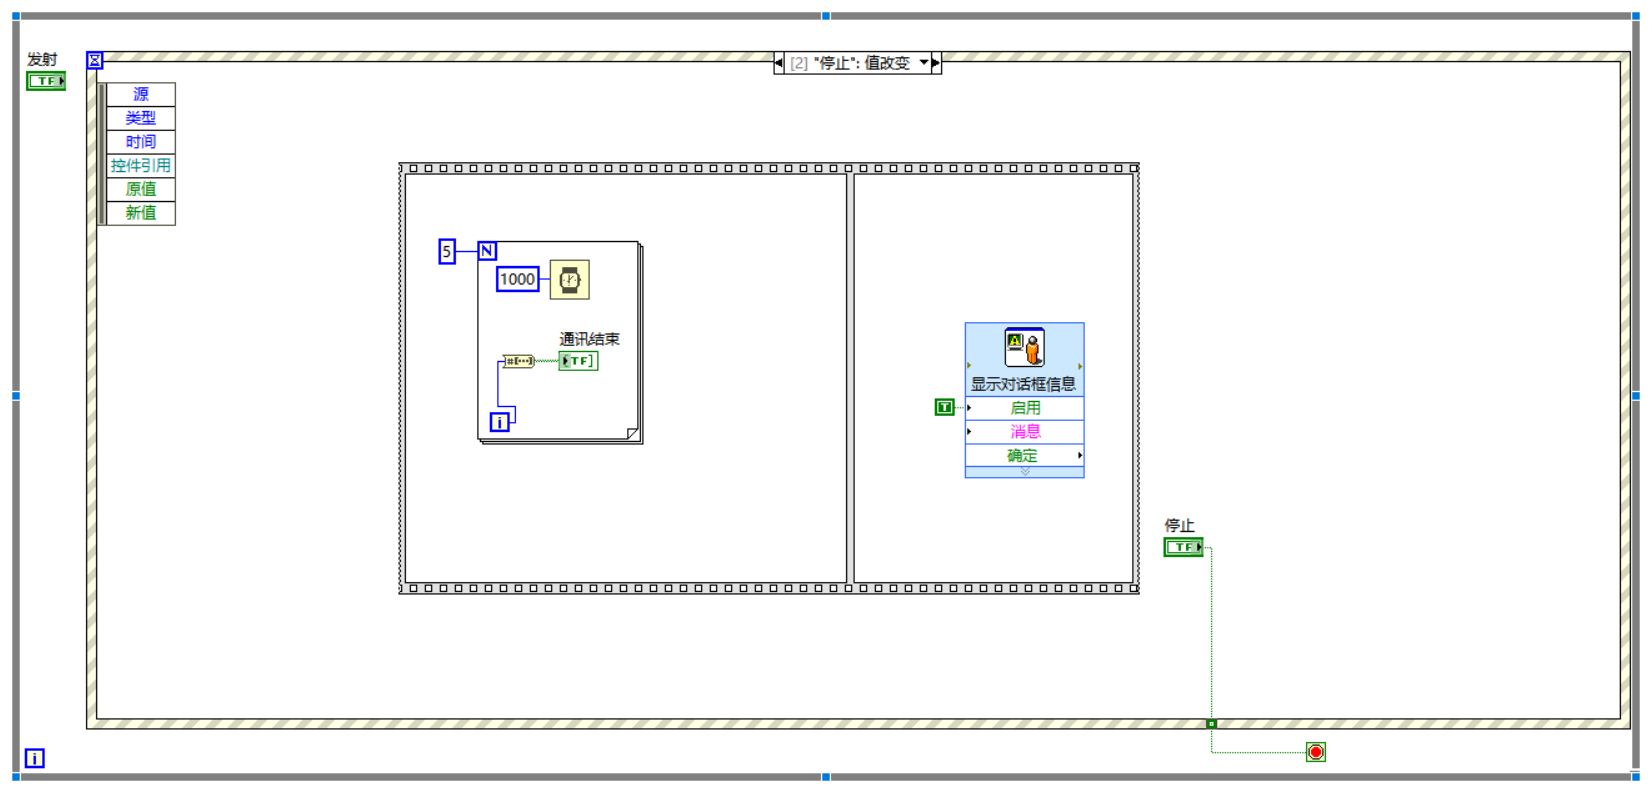
\includegraphics[width=1\textwidth]{figure/发射模块-程序2.png} 
    \caption{发射模块程序图[2]} % caption是图片的标题
    % \label{img} % 此处的label相当于一个图片的专属标志,目的是方便上下文的引用
\end{figure}
在发送模块的程序实现中,使用了while循环和for循环来执行主要功能,同时可以通过改变发射按键和停止按键的值来改变事件。与采集部分相同,此处同样使用VISA来实现串口通信。在界面的设计上,使用了数值输入控件获取数据输入,使用波形图控件用于显示激励信号等,方便用户对数据进行修改和查看。

%%%
\subsubsection{主界面的实现}
主界面的LabVIEW程序如下:
\begin{figure}[H]
    \centering % 居中 
    % 图片文件的相对路径
    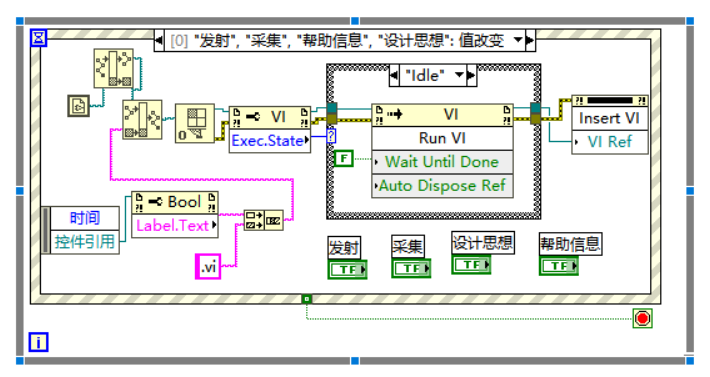
\includegraphics[width=1\textwidth]{figure/主界面-程序0.png} 
    \caption{主界面程序图[0]} % caption是图片的标题
    % \label{img} % 此处的label相当于一个图片的专属标志,目的是方便上下文的引用
\end{figure}
\begin{figure}[H]
    \centering % 居中 
    % 图片文件的相对路径
    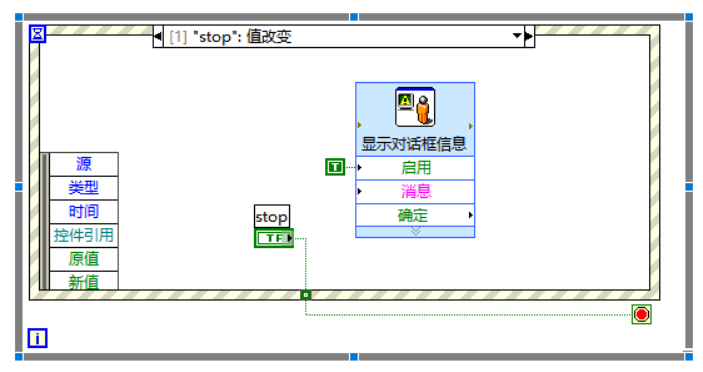
\includegraphics[width=1\textwidth]{figure/主界面-程序1.png} 
    \caption{主界面程序图[1]} % caption是图片的标题
    % \label{img} % 此处的label相当于一个图片的专属标志,目的是方便上下文的引用
\end{figure}
主界面的程序完成的主要功能即对上述两个功能模块的子VI调用,以及其他的辅助功能实现,如对所调用程序进行关停,以及提供一些与系统相关的帮助信息等。

%
\section{实习总结与心得}
%%
\subsection{实习总结}
在本次实习中,我们使用基于LabVIEW语言开发的上位机系统、51单片机系统和自制的功率驱动电路,构建了一个功能相对完整的电法勘探地学虚拟仪器,可以实现在土壤环境下对金属等低电阻率物质的勘探,在地学勘探中具有一定的应用价值。

%%
\subsection{心得与体会}
经过这次实习,我认识到基于LabVIEW的虚拟仪器开发是一个非常综合型的任务。它不仅涉及到对LabVIEW程序开发技能的掌握,还涉及到以单片机为代表的嵌入式系统的设计与应用。此外,在构建一个完整虚拟仪器系统的过程中,为了实现微弱信号的采集与数据处理等繁杂的工作,还往往需要设计特定的硬件电路以实现这些必须的功能。

整体来说,本次虚拟仪器实习是较为简单的。但是在实习的过程中,我们仍然遇到了一些问题,比如LabVIEW上位机无法和单片机建立通讯,在本应检测到金属物体时采集到的信号没有明显变化等等。对此我的一些心得是,普遍来讲,在系统设计与开发过程中遇到问题是在所难免的,重要的是不要抱有畏难情绪,而要让自己冷静下来思考问题的解决方法。同时要善于利用周边的学习资源,比如老师和同学等,都是我们学到新技能的重要来源。

\end{document}